\documentclass[12pt]{article}
\usepackage[margin=1in]{geometry} 
\usepackage{amsmath,amsthm,amssymb,amsfonts}
\usepackage{enumitem}
\usepackage{placeins}
\usepackage{mathtools, eucal}
\usepackage{graphicx}
\usepackage{color}
 

 
\begin{document}
 
%\renewcommand{\qedsymbol}{\filledbox}
%Good resources for looking up how to do stuff:
%Binary operators: http://www.access2science.com/latex/Binary.html
%General help: http://en.wikibooks.org/wiki/LaTeX/Mathematics
%Or just google stuff
 
\title{Homework 5 Solutions}
\author{Zheming Gao}
\maketitle

\section*{Problem 1 (3.1)}

Suppose $A\in\mathbb R^{m\times n}, b\in\mathbb R^m$. Add slack variables$s_1, \dots, s_m \geqslant 0$ on each row and make it a standard form. 

Let starting feasible solution be $(x_1, \dots, x_n, s_1, \dots, x_m)^T = (0, \dots, 0, b_1, \dots, b_m)^T$.




\section*{Problem 2 (3.2)}
\begin{enumerate}
\item [(a)]

\begin{proof}

Let $d$ be a feasible direction at point $x\in P$. Then, there exists $\lambda> 0$ such that $x + \lambda d \in P$, which implies $A(x + \lambda d) = b$. Since $Ax = b$, we know that $\lambda Ad = 0$ and this implies $Ad = 0$.

\end{proof}


\item [(b)]

\begin{proof}

let $d = (d_1, \dots, d_n)^T$ be a feasible direction at $x$. Let $\alpha = \min\{\frac{x_i}{-d_i} | d_i < 0, i = 1, \dots, n \}$. If $d \geqslant 0$, then let $\alpha = 1$.

It is clear that $\alpha > 0$ and $x + \alpha d \geqslant 0$.

\end{proof}

\end{enumerate}


\section*{Problem 3 (3.3)}

$$
\begin{aligned}
\text{Minimize} \qquad & -2x_1 - x_2 + x_3 + x_4 + 2x_5 &  \\
\text{subject\  to} \qquad & -2x_1 + x_2 + x_3 + x_4 + x_5 & = 12\\
 & -x_1 + 2x_2 + x_4 - x_5 & = 5 \\
 & x_1 - 3x_2 + x_3 + 4x_5 & = 11 \\
 & x_1, x_2, x_3, x_4, x_5 & \geqslant 0
\end{aligned}
$$

Here, $A = \begin{pmatrix}
-2 & 1 & 1 & 1 & 1 \\
-1 & 2 & 0 & 1 & -1 \\
1 & -3 & 1 & 0 & 4 
\end{pmatrix}$ and $b = \begin{pmatrix}
12 \\ 
5 \\
11
\end{pmatrix}$

\begin{enumerate}[label = (\alph*)]
\item 

$B = [A_3, A_4, A_5] = \begin{pmatrix}
1 & 1 & 1\\
0 & 1 & -1 \\
1 & 0 & 4
\end{pmatrix}$, and $N = [A_1, A_2] = \begin{pmatrix}
-2 & 1 \\
-1 & 2 \\
1 & -3
\end{pmatrix}$.

The fundamental matrix $M = \begin{bmatrix}
B & N \\
\textbf{0} & I
\end{bmatrix} = \begin{bmatrix}
1 & 1 & 1 & -2 & 1 \\
0 & 1 & -1 & -1 & 2 \\
1 & 0 & 4 & 1 & -3 \\
0 & 0 & 0 & 1 & 0 \\
0 & 0 & 0 & 0 & 1
\end{bmatrix}$ and $M^{-1} = \begin{bmatrix}
B^{-1} & -B^{-1} N \\
\textbf{0} & I
\end{bmatrix} = \begin{bmatrix}
2 & -2 & -1 & 3 & -1 \\
-1/2 & 3/2 & 1/2 & 0 & -1 \\
-1/2 & 1/2 & 1/2 & -1 & 1 \\
0 & 0 & 0 & 1 & 0 \\                                        
0 & 0 & 0 & 0 & 1
\end{bmatrix}$.

\item

%%Solved by matlab: rref([B, N])
Apply Gaussian elimination on matrix $[B, N]$ and get reduced row rechelon form
$$
\begin{bmatrix}
     1  &   0     &  0  &  -3  &   1 \\
     0  &   1 &    0  &   0  &   1 \\
     0  &   0 &    1  &   1  &  -1
     \end{bmatrix}
$$

Hence, $x_3 = 3x_1 - x_2 + 3, x_4 = -x_2 + 7, x_5 = -x_1 + x_2 + 2 $. Reform the LP problem using only two variables as the following:

$$
\begin{aligned}
\text{Minimize} \qquad & -x_1 - x_2 (+14) &  \\
\text{subject\  to} \qquad & 3x_1 - x_2 + 3 & \geqslant 0\\
 & -x_2 + 7 & \geqslant 0 \\
 & -x_1 + x_2 + 2 & \geqslant 0 \\
 & x_1, x_2 & \geqslant 0
\end{aligned}
$$

\item

The feasible domain is part of the intersection of three hyperplanes on $\mathbb R^5$, hence, its dimension is reduced by 3 and can be represented in $\mathbb R^2$.

We plot the region of $P$.

 \begin{figure}[htbp]
  \caption{Region $P$.}
  \centering
    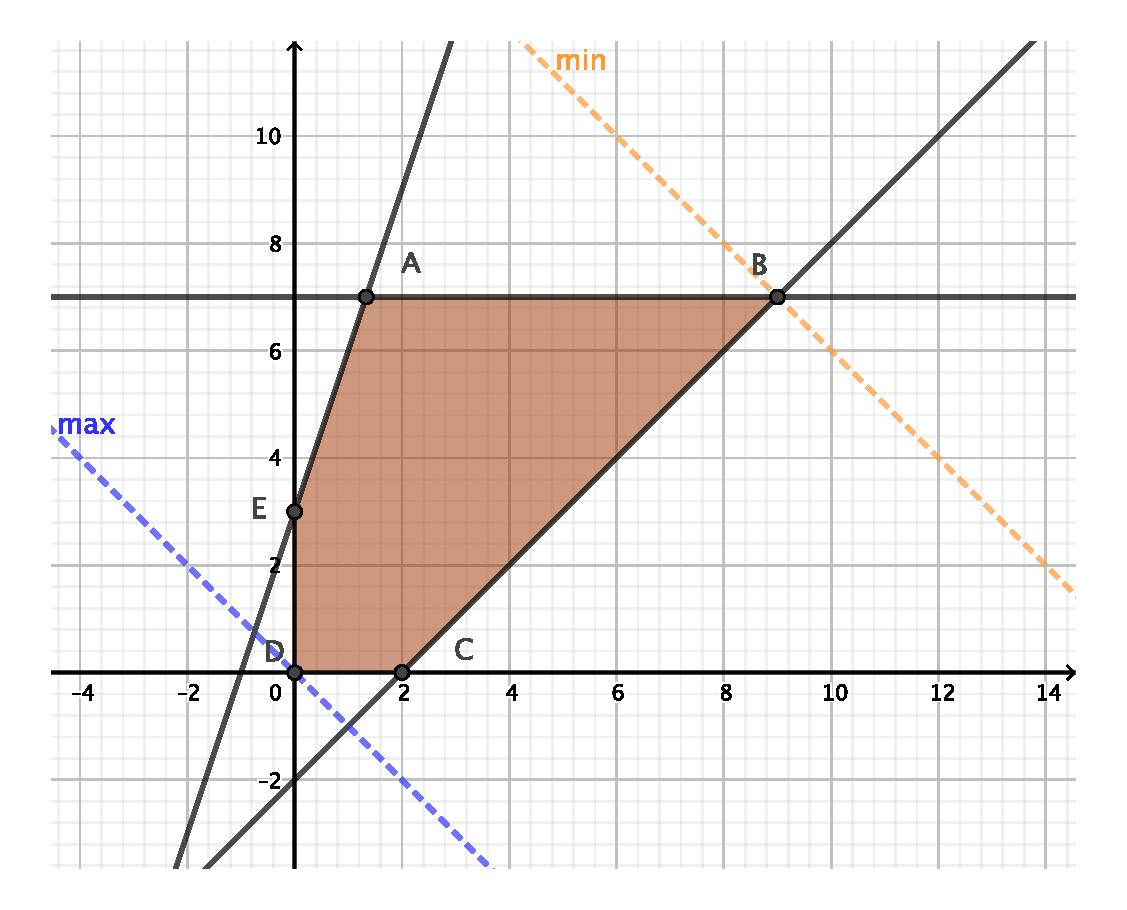
\includegraphics[width=0.5\textwidth]{problem3.pdf}
    \label{problem3}
 \end{figure}

\FloatBarrier


\item

Basic feasible solution  $\textbf x = (0,0, 3,7,2)^T$. And it is corresponding to point $D = (0,0)^T$ on fig.\ref{problem3}.

\item

$$
B^{-1}A = \begin{bmatrix}
    -3 &    1 &    1 &    0 &    0 \\
     0  &   1  &   0   &  1   &  0 \\
     1   & -1  &   0  &   0  &   1
\end{bmatrix},  \qquad
B^{-1}b = \begin{bmatrix}
3 \\ 7 \\ 2
\end{bmatrix}
$$

One explaination of this:

We see that $B^{-1}A$ is the same with the reduced row echelon form of $A$. And $B^{-1}b$ is exactly the basic feasible solution (positive entries). This is always true since

$$
Ax = b \Leftrightarrow [B | N]\begin{bmatrix}
x_B \\ x_N
\end{bmatrix} = b.
$$

Since $x_N = 0$, we get $Bx_B = b$ so that $x_B = B^{-1}b$. This implies that $B^{-1}A$ is the reduced row echelon form of $A$ for basic variable, since $B^{-1}Ax = B^{-1}b = x_B$.

(Other proper answers will be also acceptable).

\item

From $M^{-1}$ we know that $\textbf d^1 = (3,0,-1,1,0)^T$ and $\textbf d^2 = (-1,-1,1,0,1)^T$. Reduced costs:

$$
r^1 = [c_B^T|c_N^T]\textbf d^1 = (1,1,2,-2,-1)\textbf d^1 = -1, \qquad r^2 = [c_B^T|c_N^T]\textbf d^2 = (1,1,2,-2,-1)\textbf d^2 = -1
$$

\item

From above, either direction leads to a potential reduction in the objective value, since $r^1$ and $r^2$ are both negative. Consider the nonnegativity constraint($x + \alpha \textbf d \geqslant 0$), we get the step length for $\textbf d^1$ is $\alpha_1 = 2$ and for $\textbf d^2$ is $\alpha_2 = 3$.

\item
\begin{enumerate}
\item[1)] If we take $\textbf d^1$, then the new solution will be $\overline{x} = x + \alpha_1 \textbf d^1 = (0,0,3,7,2)^T  + 2(1,0,3,0,-1)^T = (2,0,9,7,0)^T \geqslant 0$. The basis now is $\overline{B} = [A_3, A_4, A_1]$ and $\overline{N} = [A_5, A_2]$. It is easy to check that $\overline{B}\overline x = b$. Hence $\overline{x}$ is a basic feasible solution(BFS). $\overline{x}$ is also an adjacent extreme point of $x$. (On fig.\ref{problem3}, $\overline{x}$ is the point $C$)

\item[2)] If we take $\textbf d^2$, then the new solution will be $\overline{x} = x + \alpha_2 \textbf d^2 = (0,0,3,7,2)^T + 3(0,1,-1,-1,1)^T = (0,3,0,4,5)^T \geqslant 0$. The basis now is $\overline{B} = [A_4, A_5, A_2]$ and $\overline{N} = [A_3, A_1]$. It is easy to check that $\overline{B}\overline x = b$. Hence $\overline{x}$ is a basic feasible solution(BFS). $\overline{x}$ is also an adjacent extreme point of $x$. (On fig.\ref{problem3}, $\overline{x}$ is the point $E$)

\end{enumerate}

\item

\begin{enumerate}
\item[1)] If we take $\textbf d^1$, update $\tilde{M} = \begin{bmatrix}
\tilde B & \tilde N \\
\textbf 0 & I
\end{bmatrix}$.

$$
\tilde M = \begin{bmatrix}
     1   &  1  &  -2  &   1  &   1\\
     0  &   1   & -1  &  -1  &   2\\
     1   &  0  &   1   &  4  &  -3\\
     0   &  0  &   0   &  1   &  0\\
     0   &  0   &  0  &   0   &  1
\end{bmatrix}, \qquad 
\tilde M^{-1} = \begin{bmatrix}
     1/2   &  -1/2  &  1/2  &   -3  &  2\\
     -1/2  &   3/2   & 1/2  &  0  &   -1 \\
     -1/2   &  1/2  &   1/2   &  -1  &  1 \\
     0   &  0  &   0   &  1   &  0\\
     0   &  0   &  0  &   0   &  1
\end{bmatrix}
$$

From the last two columns of $\tilde M^{-1}$ we get $\tilde {\textbf{d}}^5 = \begin{bmatrix}
-3 \\ 0 \\ -1 \\ 1 \\ 0
\end{bmatrix}$, $\tilde {\textbf{d}}^2 = \begin{bmatrix}
2 \\ -1 \\ 1 \\ 0 \\ 1
\end{bmatrix}$.

Let $\tilde c^T = [\tilde c_B^T | \tilde c_N^T]$. We get $\tilde c^T\tilde{\textbf d}^5 = 1 > 0$, but $\tilde c^T\tilde{\textbf d}^2 = -2 < 0$. So $\tilde x$ is not an optimal solution since $\tilde{\textbf d}^2$ is a good direction of translation.



\item[2)] If we take $\textbf d^2$, update $\overline{M} = \begin{bmatrix}
\overline B & \overline N \\
\textbf 0 & I
\end{bmatrix}$.

$$
\overline M = \begin{bmatrix}
     1  &   1  &   1  &   1   & -2\\
     1  &  -1  &   2  &   0  &  -1\\
     0   &  4  &  -3  &   1  &   1\\
     0  &   0  &   0  &   1  &   0\\
     0   &  0  &   0  &   0  &   1
\end{bmatrix}, \qquad 
\overline M^{-1} = \begin{bmatrix}
     -5/2   &  7/2  &  3/2  &   1  &  -3\\
     3/2  &   -3/2   & -1/2  &  -1  &   2 \\
     2   &  -2  &   -1  &  -1  &  3 \\
     0   &  0  &   0   &  1   &  0\\
     0   &  0   &  0  &   0   &  1
\end{bmatrix}
$$

From the last two columns of $\overline M^{-1}$ we get $\overline {\textbf{d}}^5 = \begin{bmatrix}
1 \\ -1 \\ -1 \\ 1 \\ 0
\end{bmatrix}$, $\overline {\textbf{d}}^2 = \begin{bmatrix}
-3 \\ 2 \\ 3 \\ 0 \\ 1
\end{bmatrix}$.

Let $\overline c^T = [\overline c_B^T | \overline c_N^T]$. We get $\overline c^T\overline{\textbf d}^3 = 1 > 0$, but $\overline c^T\overline{\textbf d}^1 = -4 < 0$. So $\overline x$ is not an optimal solution since $ \overline {\textbf d}^1$ is a good direction of translation.
\end{enumerate}

\item 
\begin{enumerate}
\item [1)]
If basic varialbes are $x_3, x_4, x_1$, then the reduced row echelon form (RREF) of $[\tilde{B}, \tilde N, -b]$ is

$$
\begin{bmatrix}
     1  &   0   &  0  &   3 &   -2  &  -9\\
     0  &   1  &   0  &   0 &    1  &  -7\\
     0  &   0   &  1  &   1 &   -1  &  -2
\end{bmatrix}
$$

and $x_3 = 2x_2 - 3x_5 + 9, x_4 = -x_2 + 7, x_1 = x_2 - x_5 + 2 $. Reform the LP problem using only two variables as the following:

$$
\begin{aligned}
\text{Minimize} \qquad & -2x_2 + x_5 (+12) &  \\
\text{subject\  to} \qquad & 2x_2 - 3x_5 + 9 & \geqslant 0\\
 & -x_2 + 7 & \geqslant 0 \\
 & x_2 - x_5 + 2 & \geqslant 0 \\
 & x_2, x_5 & \geqslant 0
\end{aligned}
$$

We plot the region.

 \begin{figure}[htbp]
  \caption{Region on $x_2, x_5$.}
  \centering
    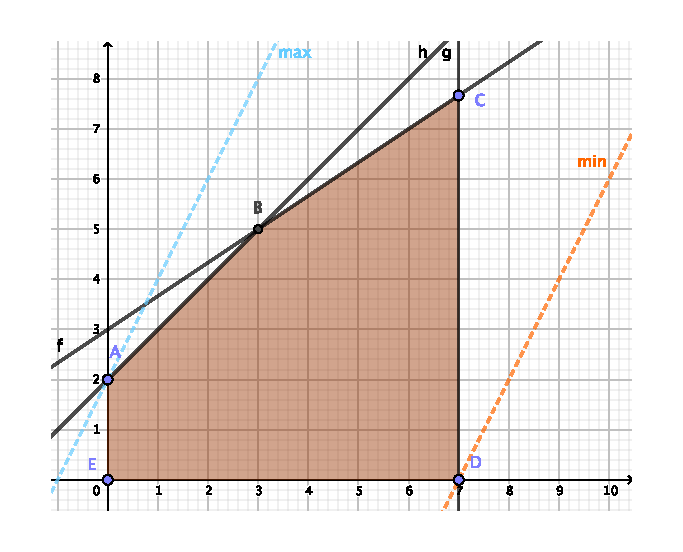
\includegraphics[width=0.5\textwidth]{problem3_j1.pdf}
    \label{problem3j1}
 \end{figure}

\FloatBarrier



\item [2)]

If basic varialbes are $x_4, x_5, x_2$, then the reduced row echelon form (RREF) of $[\overline{B}, \overline N, -b]$ is

$$
\begin{bmatrix}
     1  &   0  &   0  &  -1  &   3  &  -4 \\
     0  &   1  &   0   &  1  &  -2 &   -5\\
     0  &   0  &   1   &  1  &  -3  &  -3
\end{bmatrix}
$$

and $x_4 = x_3 - 3x_1 + 4, x_5 = -x_3 + 2x_1 + 5, x_2 = -x_3 + 3x_1 + 3 $. Reform the LP problem using only two variables as the following:

$$
\begin{aligned}
\text{Minimize} \qquad & -4x_1 + x_3 (+11) &  \\
\text{subject\  to} \qquad & x_3 - 3x_1 + 4 & \geqslant 0\\
 & -x_3 + 2x_1 + 5 & \geqslant 0 \\
 & -x_3 + 3x_1 + 3 & \geqslant 0 \\
 & x_1, x_3 & \geqslant 0
\end{aligned}
$$

We plot the region.

 \begin{figure}[htbp]
  \caption{Region on $x_1, x_3$.}
  \centering
    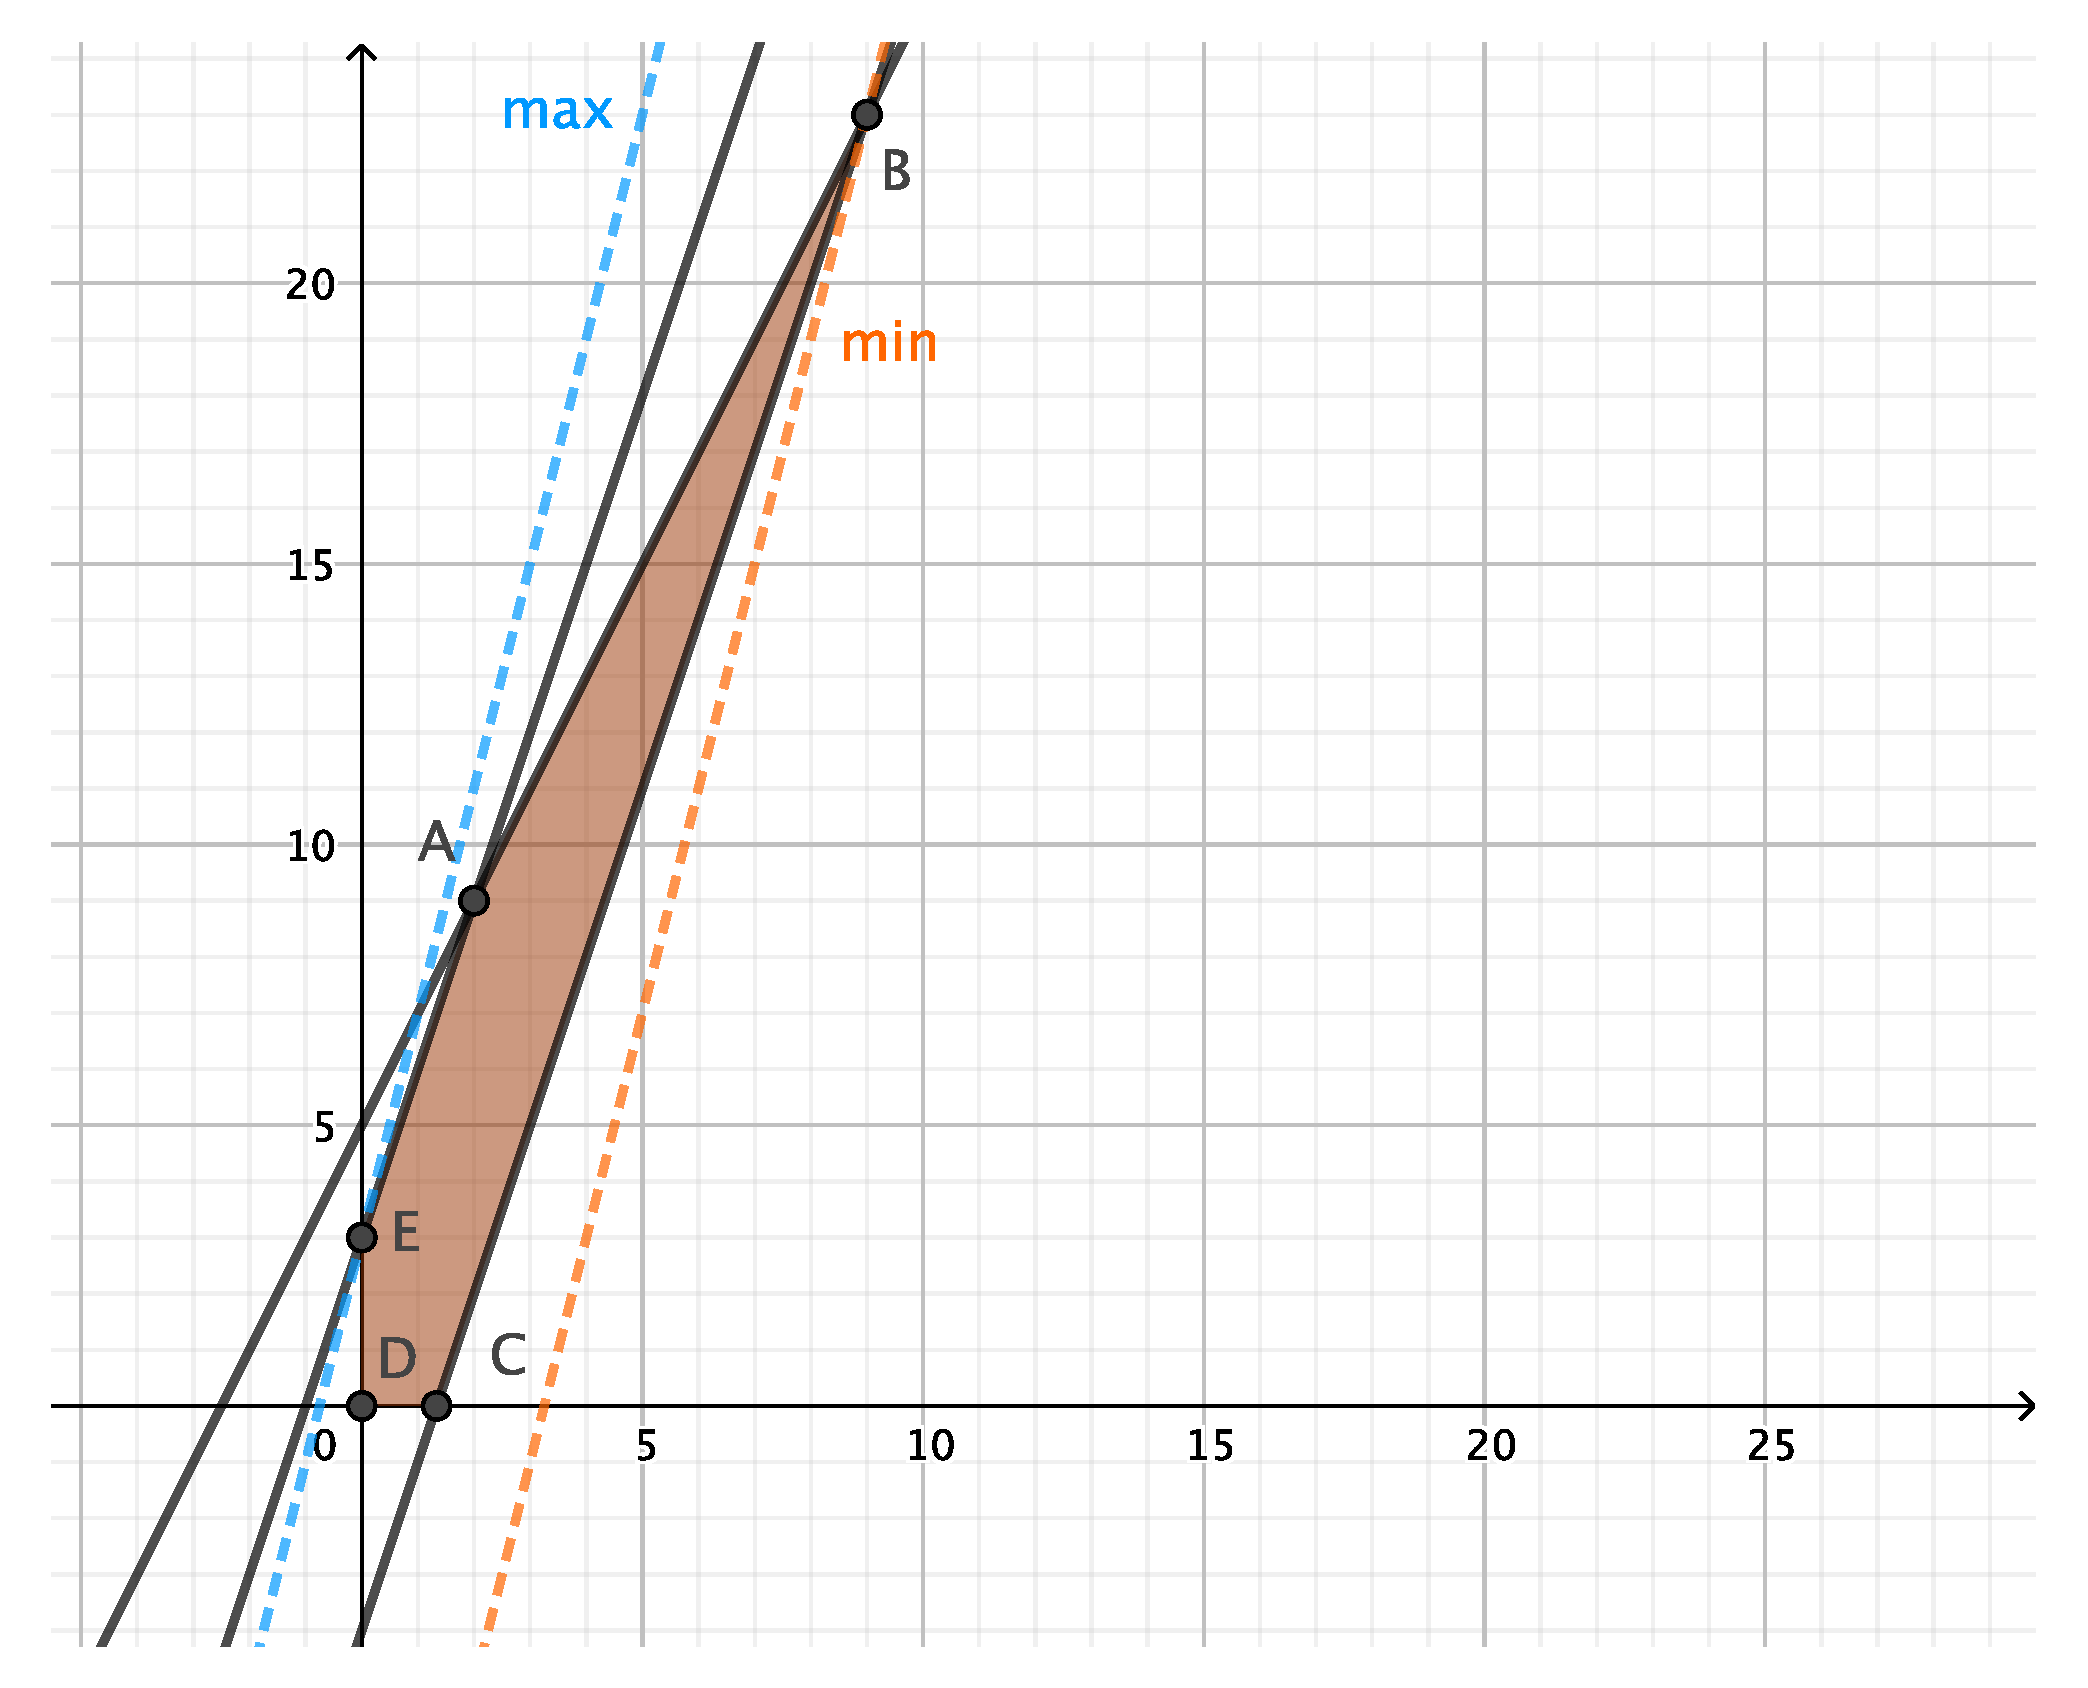
\includegraphics[width=0.5\textwidth]{problem3_j2.pdf}
    \label{problem3j2}
 \end{figure}

\FloatBarrier

\end{enumerate}

\item

(Any proper answer will be acceptable).

\item

We can always express $n-2$ variables by using the rest $2$ variables. Then, the LP problem can be reformed as an LP problem on $\mathbb R^2$.



\end{enumerate}



\section*{Problem 4 (3.4)}

From point $x = [1/2, 0, 0, 0, 1, 1]^T$, we know that $B = [A_5, A_6, A_1]$ and $N = [A_2, A_3, A_4]$. Construct matrix $M = \begin{bmatrix}
B & N \\
\textbf 0 & I
\end{bmatrix}$ and reduced cost $r = c_N^T - c_B^TB^{-1}N = [-1, -1, 1/2]$.

Note that $r_2, r_3$ are negative, and figure out the step length $\alpha_2 = \alpha_3 = 1/2$. Hence, we can pick either one from $\textbf d^2$ or $\textbf{d}^3$. Let's pick $\textbf d^2$. $x_{\text{new}} = x + \alpha_2\textbf{d}^2 = [1/2,1/2,0,0,0,1]^T$. 

Next step:

From point $x =  [1/2,1/2,0,0,0,1]^T$, we know $B = [A_2, A_6, A_1]$ and $N = [A_5, A_3, A_4]$. Construct matrix $M$ and reduced cost $r = c_N^T - c_B^TB^{-1}N = [1/2, -1, 1/2]$. Find the negative direction, pick $\textbf d^3$ with $\alpha_3 = 1/2$. $x_{\text{new}} = x + \alpha_3\textbf{d}^3 =  [1/2, 1/2, 1/2, 0, 0, 0]^T$.

Next step:

From point $x = [1/2, 1/2, 1/2, 0, 0, 0]^T$, we know $B = [A_1, A_2, A_3]$ and $N = [A_4, A_5, A_6]$. Compute the reduced cost $r = c_N^T - c_B^TB^{-1}N = [1/2, 1/2, 1/2]  \geqslant 0$. Hence, $x = [1/2, 1/2, 1/2, 0, 0, 0]^T$ is the optimal solution.



\section*{Problem 5 (3.8)}

\begin{proof}

For a degenerate BFS $x$ with $p(<m)$ positive components, we have $n-p$ zero components in it. And also, $n-m$ of $n-p$ will be nonbasic variables and there will be at most $C(n-p, n-m)$ situations. 

\end{proof}


\section*{Problem 6 (3.9)}

\begin{proof}

We know $\overline{M} = \begin{bmatrix}
 B & N \\
\textbf 0 & I
\end{bmatrix}$ and let $W = \begin{bmatrix}
 B^{-1} & -B^{-1}N \\
\textbf 0 & I
\end{bmatrix} \in \mathbb{R}^{n\times n}$. Thus, it is enough to check $W\overline M = I$ and $\overline M W = I$.

Those are true since

$$
W\overline M = \begin{bmatrix}
B^{-1}B - B^{-1}N\textbf 0 & B^{-1}N - B^{-1}NI \\
\textbf 0 B + I \textbf 0 & \textbf 0 N + I*I
\end{bmatrix} \qquad = \begin{bmatrix}
I & \textbf 0 \\
\textbf 0 & I
\end{bmatrix}
$$. 

Similarly, $\overline M W = I$. 

In conclusion, $\overline{M}^{-1} = W$.

\end{proof}

\section*{Problem 7 (3.13)}

From point $x = [x_1, x_2, x_3, x_4]^T = [30, 0, 10, 0]^T$, we know that $B = [A_3, A_1]$ and $N = [A_2, A_4]$. Compute reduced cost $r = c_N^T - c_B^TB^{-1}N = [-1/2, 3/2]$.

Note that $r_2$ is negative, so $x_2$ enter the basis. Construct $M^{-1} = \begin{bmatrix}
1 & -1/2 & -1/2 & 1/2 \\
0 & 1/2 & -1/2 & -1/2 \\
0 & 0 & 1 & 0  \\
0 & 0 & 0 & 1 
\end{bmatrix}$ to figure out $\textbf d^2 = [-1/2, 1, -1/2, 0]^T$  and the step length $\alpha_2 = 20$ . Hence, $x_{\text{new}} = x + \alpha_2\textbf{d}^2 = [20, 20, 0, 0]^T$. 

Next step:

From point $x = [x_1, x_2, x_3, x_4]^T = [20, 20, 0, 0]^T$, we know that $B = [A_1, A_2]$ and $N = [A_3, A_4]$. Compute reduced cost $r = c_N^T - c_B^TB^{-1}N \geqslant 0$. Hence, this is the optimal solution. The optimal value $z^* = c^Tx^* = -100 $.



\section*{Problem 8 (3.14)}

From point $x = [x_1, x_2, x_3, x_4, x_5]^T = [30, 0, 10, 0, 0]^T$, we know that $B = [A_3, A_2, A_1]$ and $N = [A_4, A_5]$. Compute reduced cost $r = c_N^T - c_B^TB^{-1}N = [2, -3]$.

Note that $r_5$ is negative, so $x_5$ enter the basis. Construct $M^{-1} = \begin{bmatrix}
1 & -1 & 1 & 1 & -1 \\
0 & 1 & -2 & -1 & 2 \\
0 & 0 & 1 & 0 & -1 \\
0 & 0 & 0 & 1 & 0 \\
0 & 0 & 0 & 0 & 1
\end{bmatrix}$ to figure out $\textbf d^5 = [-1, 2, -1, 0, 1]^T$  and the step length $\alpha_5 = 10$ . Hence, $x_{\text{new}} = x + \alpha_5\textbf{d}^5 = [20, 20, 0, 0, 10]^T$. 

Next step:

From point $x = [x_1, x_2, x_3, x_4, x_5]^T = [20, 20, 0, 0,  10]^T$, we know that $B = [A_1, A_2, A_5]$ and $N = [A_3, A_4]$. Compute reduced cost $r = c_N^T - c_B^TB^{-1}N \geqslant 0$. Hence, this is the optimal solution. The optimal value $z^* = c^Tx^* = -100 $.



\end{document}